\section{Module 6. Diffusion tensor imaging}

\textbf{Preprocessing and Module I/O}

In order to improve diffusion tensor estimation it is imperative to
remove artifacts. In addition to standard MRI pre-processing, one
needs to correct for artifacts arising the use of diffusion-gradient
pulse sequences and longer acquisition time. While hardware manufacturers
try to proactively diminish some of these effects, software processing
is still mandatory. 
\hfill\\

\textbf{Module Input}:
\begin{itemize}
	\item 
	3D structural data array of shape X x Y x Z, where XY - pixel image intensities, Z - chosen slice, which is the T1- or T2-weighted image corresponding the the given DWI acquisition
	
	\item 
	4D diffusion data array of shape X x Y x Z x M, where XY - pixel image intensities, Z - chosen slice, M - applied diffusion gradient direction
	
	\item 
	b\_value, a scalar value corresponding to applied diffusion gradient sequence magnitude
	
	\item 
	2D gradients matrix of shape M x 3, where each row corresponds to a normalized $(x,y,z)$ components of diffusion gradient sequence vectors
		
	\item 
	optionally - 3D binary mask of shape X x Y x Z, corresponding to the brain area detected by Module 8 (Skull Stripping); if not supplied, DTI is computed on each input data voxel

\end{itemize}
\hfill

\textbf{Module Output}:
\begin{itemize}
	\item
	list of size Z, corresponding to each slice; each list element is a dictionary of biomarker images: MD, RA, FA, VR of shape X x Y, and biomarker FA\_rgb of shape X x Y x 3
\end{itemize}


\subsection{NLS tba}

Autorzy wyżej wymienionej publikacji proponują modyfikację tej zależności tak, aby:
\begin{equation}
\boldsymbol{\delta}=-\left(\nabla^2{f_{NLS}}+\lambda \boldsymbol{I}\right)^{-1}\nabla{f_{NLS}}
\label{Eq:m6_eq_22}
\end{equation}
gdzie $\lambda$ jest niezerowym parametrem algorytmu Levenberg-Marquardt, zaś $\boldsymbol{I}$ to macierz jednostkowa.

Schemat blokowy omawianej metody (Modified Newton's Method) przedstawiony został na rysunku \ref{fig:m6_pic_1}.

\begin{figure}[!h]
	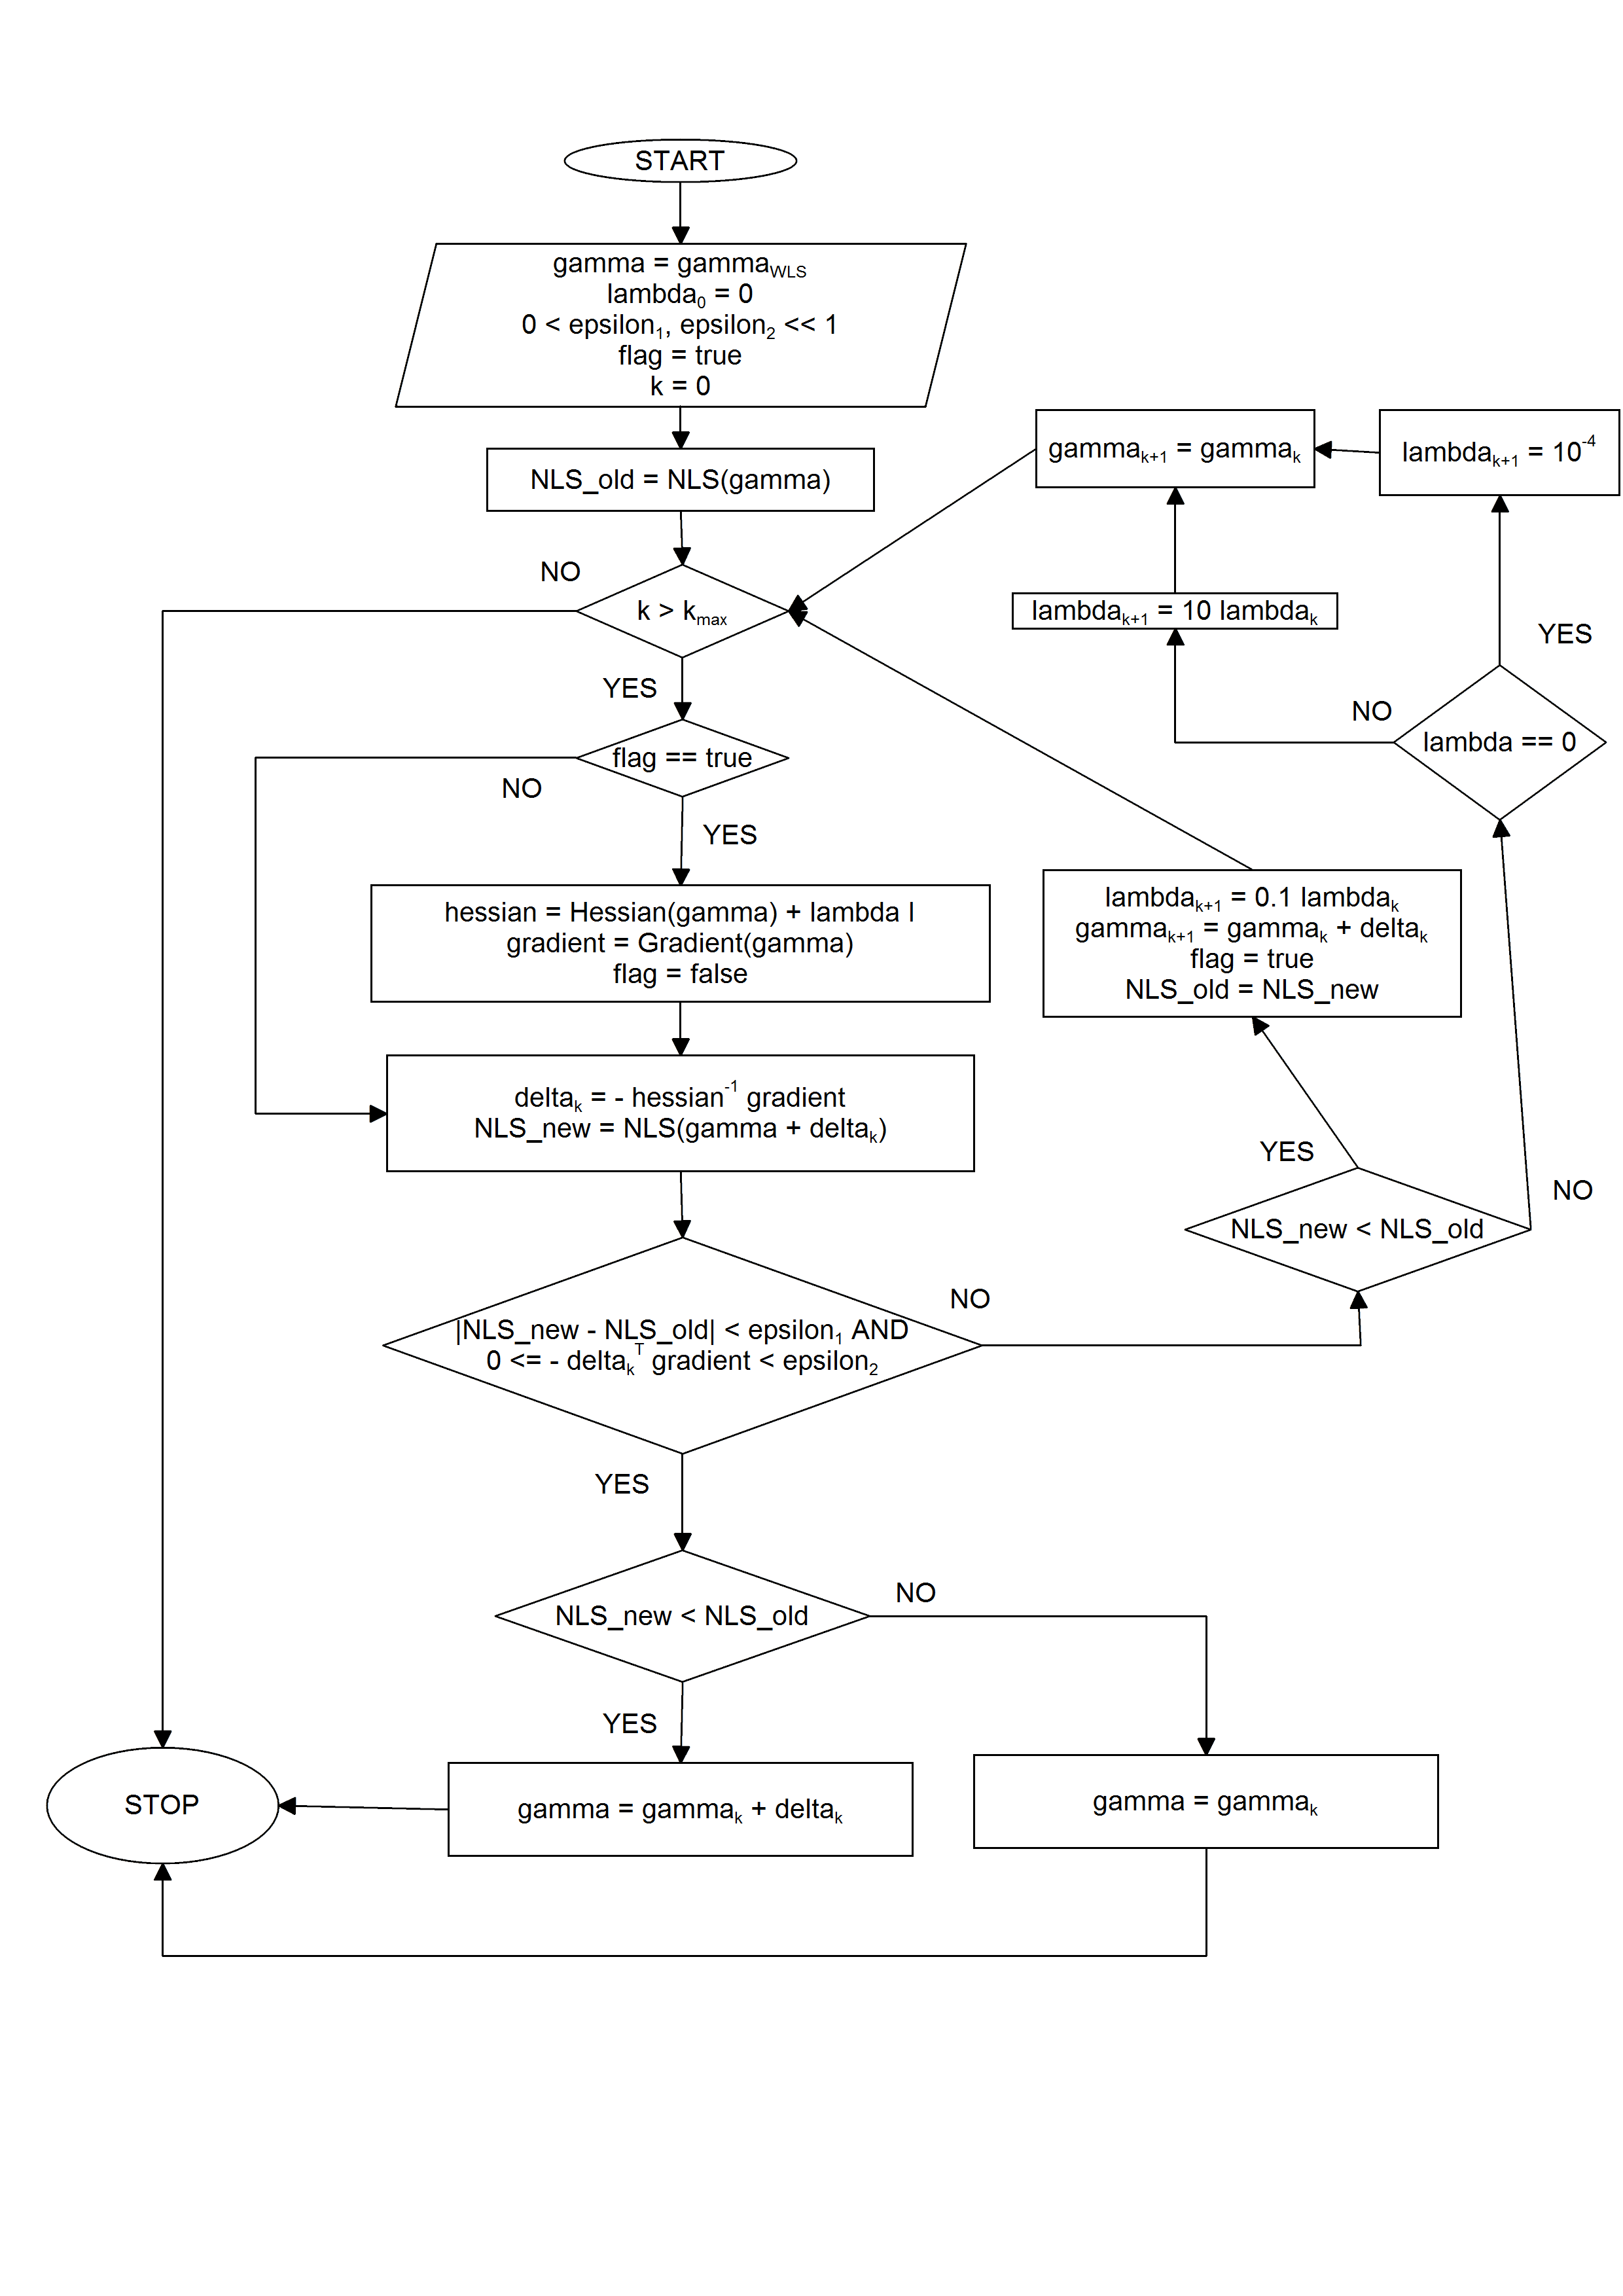
\includegraphics[width=8cm]{figures/Module_06/mfn}
	\centering
	\caption{Zmodyfikowany algorytm Newtona do wyznaczania minimum funkcji NLS (na bazie \cite{m6_koay2006a})}.
	\label{fig:m6_pic_1}
\end{figure}